%!TEX TS-program = xelatex
%!TEX encoding = UTF-8 Unicode

\documentclass[12pt]{article}
\usepackage{geometry}                % See geometry.pdf to learn the layout options. There are lots.
\geometry{a4paper,top=2cm}
\usepackage[parfill]{parskip}    % Activate to begin paragraphs with an empty line rather than an indent
\usepackage{graphicx}
\usepackage{amsmath}
\usepackage{amssymb}
\usepackage{mathtools}
\usepackage{physics}
\newcommand{\be}{\begin{equation}}
\newcommand{\ee}{\end{equation}}
\usepackage[thicklines]{cancel}
\usepackage{url}
\usepackage{booktabs}
\usepackage{qcircuit}
\usepackage{circledsteps}

\usepackage{fontspec,xltxtra,xunicode}
\defaultfontfeatures{Mapping=tex-text}

\newcommand{\polv}{\ensuremath{\updownarrow}}
\newcommand{\polh}{\ensuremath{\leftrightarrow}}
\newcommand{\poldr}{\rotatebox[origin=c]{45}{\ensuremath{\leftrightarrow}}}
\newcommand{\poldl}{\rotatebox[origin=c]{-45}{\ensuremath{\leftrightarrow}}}

\title{Advanced Quantum Mechanics\\Class 17}
%\author{The Author}
\date{October 04, 2022}                                           % Activate to display a given date or no date

\setcounter{section}{6}
\setcounter{subsection}{4}
\setcounter{equation}{44}

\begin{document}
\maketitle

%%% 01 OKAY
\subsection{Conservation laws (continued)}

\subsubsection{Translations}
 
Start with one-dimensional coordinate space, x-axis.
Let $\hat{X}$ be position operator, and $\ket{\varphi}$ a state
that describes a particle \emph{localized} in the neighborhood
of a point $x_0$ on the x-axis with a \emph{dispersion} $\Delta x$:
\begin{gather}
\bra{\varphi}\hat{X}\ket{\varphi} = \ev*{\hat{X}} = x_0\\
\bra{\varphi}(\hat{X}-x_0)^2\ket{\varphi} = (\Delta x)^2
\end{gather}

%%% 02 OKAY
\begin{center}
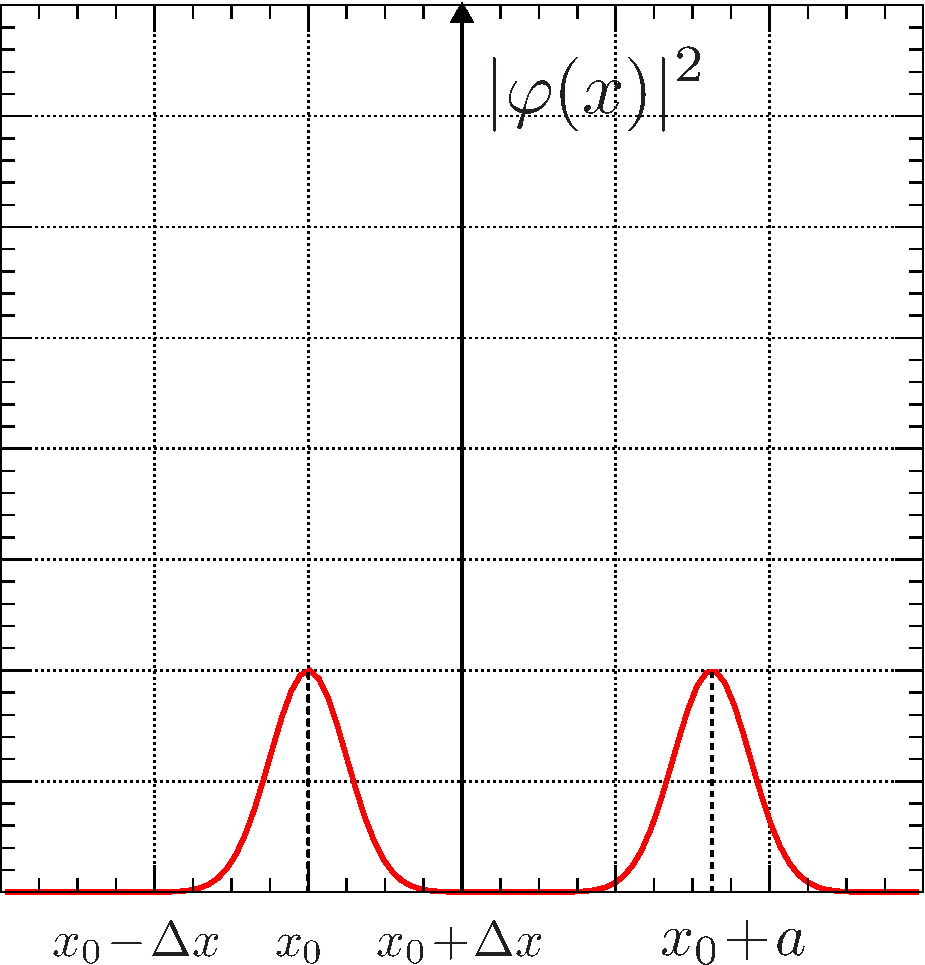
\includegraphics[width=0.5\textwidth]{Figures/translation.pdf}
\end{center}
Let us apply to $\ket{\varphi}$ a translation by $a$:
\begin{align}
\ket{\varphi} \rightarrow \ket{\varphi_a} 
&= e^{-i/\hbar a \hat{P}} \ket{\varphi},\, \hat{P} = \hat{P}_x \rightarrow \text{ momentum}\\
&= \hat{U}(a) \ket{\varphi}
\end{align}
%
$\hat{U}(a)$ is unitary:
\be
\hat{U}^{-1}(a) = \hat{U}(-a) 
= \hat{U}^{\dagger}(a) = e^{i/\hbar a \hat{P}}
\ee

After the translation, particle is localized around the
point $x_0 + a$, with dispersion $\Delta x$.
We use the correspondence principle:
\be
\begin{aligned}
\ev*{\hat{X}}_a
&= x_0+a = \ev*{\hat{X}} + a 
= \bra{\varphi}\hat{X}+a\ket{\varphi}\\
&=\bra*{\hat{U}(a)\varphi}\hat{X}\ket*{\hat{U}(a)\varphi}\\
&=\bra{\varphi}\hat{U}^{-1}(a)\hat{X}\hat{U}(a)\ket{\varphi}
\end{aligned}
\ee
but $\ket{\varphi}$ is arbitrary,
\be
\hat{U}^{-1}(a)\hat{X}\hat{U}(a) = \hat{X} + a
\label{eq:g51}
\ee
Expanding $\hat{U}(a)$ for $a \to 0$:
\be
\hat{U}(a) \simeq I - \frac{i}{\hbar} a \hat{P}
\ee

%%% 03 OKAY
\be
\begin{aligned}
\left(I - \frac{i}{\hbar} a \hat{P}\right)
&\hat{X}
\left(I - \frac{i}{\hbar} a \hat{P}\right)\\
&\Downarrow \text{canonical commutation relation}\\
&[\hat{X},\hat{P}] = i\hbar I
\end{aligned}
\ee

From~\eqref{eq:g51}
, one also has:
\be
\begin{aligned}
\hat{U}^{-1}(a)\hat{X}^n\hat{U}(a) 
&=\hat{U}^{-1}(a)\hat{X}\hat{X}\ldots\hat{X}\hat{U}(a)\\
&=\underbrace{\hat{U}^{-1}(a)\hat{X}\hat{U}(a)}%
_{\hat{X}+a}
\hat{U}^{-1}(a)\hat{X}\hat{U}(a)
\ldots
\underbrace{\hat{U}^{-1}(a)\hat{X}\hat{U}(a)}%
_{\hat{X}+a}\\
&=(\hat{X}+a)^n
\end{aligned}
\ee
from which follows the result
\be
\begin{aligned}
\hat{U}^{-1}(a)f(\hat{X})\hat{U}(a) 
&= \hat{U}^{-1}(a)
[f(0) + f^\prime(0)\hat{X}^2 + \ldots]
\hat{U}(a)\\
&=f(0) + f^\prime(0)(\hat{X}+a)^2 + \ldots\\
&=f(\hat{X}+a)
\end{aligned}
\label{eq:g55}
\ee
For $a \to 0$, expanding both sides of \eqref{eq:g55}
to first order:
\[
\left(I + \frac{i}{\hbar} a \hat{P}\right) f(\hat{X}) \left(I - \frac{i}{\hbar} a \hat{P}\right) = 
f(\hat{X}) + a \frac{\partial f}{\partial\hat{X}}
\]
whence
\be
[\hat{P},f(\hat{X})] = -i\hbar\frac{\partial}{\partial\hat{X}}f(\hat{X})
\ee
%%% 04 OKAY
\setcounter{equation}{53}
Taking $f(\hat{X}) = e^{i\beta\hat{X}}$, $\beta$ real, Eq.~\eqref{eq:g55}
implies
\be
\begin{aligned}
e^{i/\hbar a\hat{P}} e^{i\beta\hat{X}} e^{-i/\hbar a\hat{P}}
&= e^{i\beta(\hat{X}+a)}\\
&= e^{i\beta\hat{X}} e^{i\beta a}
\end{aligned}
\ee
know as \emph{Weyl form} of the canonical
commutation relation; involves only the
bound operators $e^{i/\hbar a\hat{P}}$ and $e^{i\beta\hat{X}}$.

From the result
\be
(\Delta_\varphi \hat{A})(\Delta_\varphi \hat{B})
\geq \frac{1}{2} |\ev*{\hat{C}}_\varphi|
\ee
whence
\[
\begin{aligned}
\Delta_\varphi \hat{A} 
&\to \Delta x = \ev*{\hat{X}^2}_\varphi - 
\underbrace{\ev*{\hat{X}}}%
_{x}{^2_\varphi} = \ev*{(\hat{X}-x)^2}_\varphi\\
\Delta_\varphi \hat{B} 
&\to \Delta p = \ev*{\hat{P}^2}_\varphi - 
\underbrace{\ev*{\hat{P}}}%
_{p}{^2_\varphi} = \ev*{(\hat{P}-p)^2}_\varphi\\
\hat{C} 
&= \hbar I \to \ev*{\hat{C}} = \hbar
\end{aligned}
\]
and finally
\be
\boxed{\Delta x \Delta p \geq \frac{\hbar}{2}}
\ee
\emph{Exercise:} show that the canonical commutation
relations are preserved under a unitary transformation $\hat{U}$:
\be
\hat{X} \to \hat{X}^\prime = \hat{U}^{-1}\hat{X}\hat{U},\quad
\hat{P} \to \hat{P}^\prime = \hat{U}^{-1}\hat{P}\hat{U}
\ee

%%% 05 OKAY

\emph{Explicit realization} of $[\hat{X},\hat{P}] = i\hbar$ in $L^{2}(\mathbb{R})$, \textit{i.e.}
in the space of differentiable functions $\varphi(x)$ which are
square-integrable in the real line $[-\infty,\infty]$:
\begin{align}
\ket{\hat{X}\varphi} 
&\to \varphi(x) \label{eq:g58p}\\
\ket{\hat{X}\varphi} = \ket{\chi} 
&\to (\hat{X}\varphi)(x) = \chi(x) = x\varphi(x)\label{eq:g59p}\\
\ket{\hat{P}\varphi} = \ket{\psi} 
&\to \underbrace{(\hat{P}\varphi)}_{\psi}(x) = \psi(x)
= -i\hbar\frac{\partial\varphi}{\partial x}\label{eq:g60p}
\end{align}
%
Verification:
%
\be
\begin{aligned}
\left(
(\hat{X}\hat{P}-\hat{P}\hat{X})\varphi
\right)(x)
&=(\hat{X}\underbrace{\hat{P}\varphi}_{\psi})(x) - (\hat{P}\underbrace{\hat{X}\varphi}_{\chi})(x)\\
&=(\hat{X}\psi)(x) - (\hat{P}\chi)(x)\\
&=x\psi(x) - i\hbar\frac{\partial}{\partial x}(\chi(x)\\
&=x\left(- i\hbar\frac{\partial\varphi}{\partial x}\right) - 
i\hbar\frac{\partial}{\partial x}\left(x\varphi(x)\right)\\
&=i\hbar\varphi(x)\\
\end{aligned}
\ee
%
Unitary equivalence theorem of von Neumann
-- all representations of the canonical commutation
relation of the Weyl form are \emph{unitarily equivalent}
to the representation in $L^{2}(\mathbb{R})$ 
Eqs.~\eqref{eq:g58p}--\eqref{eq:g60p}.
Moreover, any operator in $H$ can be written as a
function of $\hat{X}$ and $\hat{P}$, \textit{i.e.} representation \eqref{eq:g58p} and
%%% 06 OKAY
\eqref{eq:g59p} is irreducible. Any operator that commutes
with $\hat{X}$ ($\hat{P}$) is a function of $\hat{X}$ ($\hat{P}$). Any operator that commutes with $\hat{X}$ \emph{and} $\hat{P}$ is a multiple 
of the identity operator.

Generalization to three dimensions: $x\to x,y,z$ 
\be
[\hat{X}_i, \hat{P}_j] - i\hbar \delta_{ij} I,\quad i,j = x,y,z
\ee

\subsubsection{Galilean invariance in one dimension}

Start with \emph{one spatial} dimension ($D=1$). In nonrelativistic
physics, when changing from one reference frame to another
moving with speed $v$ with respect to the first one,
the coordinates $x$ and $x^\prime$ in the respective frames
are related by (in the passive point of view):
\be
x^\prime = x-vt
\ee
In the active point of view: particles in a reference
frame are ``boosted'' by an amount $v$, \textit{i.e.} the speeds
of all particles are modified by $v$:
\be
\text{initial state: } x,\dot{x},\quad p = m\dot{x}, K = \frac{1}{2} m \dot{x}^2
\ee
where $m$ is the mass and $K$ is the kinetic energy,
\be
\text{boosted state: } x^\prime=x+vt,\dot{x}^\prime = \dot{x}+v,\quad p^\prime = m\dot{x}^\prime, K^\prime = \frac{1}{2} m \dot{x}^{\prime2}
\label{eq:g65}
\ee
%%% 07 OKAY
Classical physics: form of the equations o motion
remains invariant under boosts.\\
Quantum physics: Galilean boost is represented in
Hilbert space by a unitary operator. So
\be
\hat{U}(v) = e^{-i/\hbar v \hat{G}},\quad \hat{G} = \hat{G}^\dagger
\ee
from Stone's theorem, $\hat{G}$ is the
generator of infinitesimal
boosts. Hence
\be
\ket{\varphi} \stackrel{v}{\to} \ket{\varphi_v} = \hat{U}(v)\ket{\varphi}
\ee
%
\be
\ev*{\hat{A}}_\varphi = 
\bra{\varphi_v}\hat{A}\ket{\varphi_v} = 
\bra{\varphi}\hat{U}^{-1}(v)\hat{A}\hat{U}(v)\ket{\varphi} = 
\ee
From Eq.~\eqref{eq:g65},
one expects, for $t = 0$:
\begin{align}
\ev*{\hat{X}}_v &= \ev*{\hat{X}} \label{eq:g69}\\
\ev*{\hat{\dot{X}}}_v &= \ev*{\hat{\dot{X}}} + v \label{eq:g70}\\
\ev*{\hat{P}}_v &= \ev*{\hat{P}} + mv \label{eq:g71}
\end{align}
Since in QM, we have Heisenberg's equation:
\be
\dot{X} = \frac{i}{\hbar} [\hat{H},\hat{X}]
\ee
imposition of \eqref{eq:g70}
leads to strong constraints on
%%% 08 OKAY
the possible Hamiltonians.

Eqs.~\eqref{eq:g69}--\eqref{eq:g71} are valid for any $\ket{\varphi}$ $\to$ valid at the
operator level. Eq.~\eqref{eq:g71} $\to$
%
\be
e^{i/\hbar v \hat{G}} \hat{P} e^{-i/\hbar v \hat{G}} =
\hat{P} + m v I
\label{eq:g73}
\ee	
so when $v \to 0$:
\be
[\hat{G},\hat{P}] = -i\hbar m I
\ee
so it is possible to choose
\be
\hat{G} = -m \hat{X}
\ee
From Eq.~\eqref{eq:g70}
\be
e^{i/\hbar v \hat{G}} \hat{P} e^{-i/\hbar v \hat{G}} =
\hat{\dot{X}} + v I
\ee
and subtracting \eqref{eq:g73} from this
\be
e^{i/\hbar v \hat{G}}
\left(\hat{\dot{X}} - \frac{\hat{P}}{m}\right) 
e^{-i/\hbar v \hat{G}} =
\hat{\dot{X}} - \frac{\hat{P}}{m}
\ee
so $\hat{\dot{X}} - \frac{\hat{P}}{m}$ commutes with $\hat{G}$ and, due to
Eq.~(75), it commutes also with $\hat{X}$.

Using the von Neumann theorem:
\be
\hat{\dot{X}} - \frac{\hat{P}}{m} = \frac{1}{m} f(\hat{X})
\ee
where we made the $1/m$ factor explicit. Finally:
%%% 09 OKAY
\setcounter{equation}{77}
\be
\hat{P} = m\hat{\dot{X}} - f(\hat{X})
\ee

\fbox{\emph{(Valid in one spatial dimension only.)}} \emph{Exercise:} show that $f(\hat{X})$ can be
be eliminated by a unitary transformation 
($\equiv$ local gauge transformation).
So, without loss of generality, one can choose
\be
\hat{P} = m \hat{\dot{X}}
\label{eq:g79}
\ee

Now, let us use these results to determine the
most general form of the Hamiltonian compatible
with Galilean invariance:
\begin{itemize}
\item $\hat{K}$: kinetic energy operator, use classical physics
correspondence
\be
\hat{K} = \frac{1}{2} m \hat{\dot{X}}^2
\stackrel{\text{Eq.\,}\eqref{eq:g79}}{=} \frac{1}{2m} \hat{P}^2
\ee
\item the commutator of $\hat{K}$ with $\hat{X}$ is:
\be
[\hat{K},\hat{X}] = \frac{1}{2m}
[\hat{P}^2,\hat{X}] = -i\hbar\frac{\hat{P}}{m}
\ee
so
\be
\frac{\hat{P}}{m} = \frac{i}{\hbar} [\hat{K},\hat{X}]
\stackrel{\text{Eq.\,\eqref{eq:g79}}}{=}
\hat{\dot{X}} = \frac{i}{\hbar}[\hat{H},\hat{X}]
\ee
therefore
\be
[\hat{K}-\hat{H},\hat{X}] = 0
\ee
\end{itemize}
%%% 10 OKAY
From von Neumann theorem:
\be
\hat{K}-\hat{H} = f(\hat{X}) \equiv -V(\hat{X})
\ee
or
\be
\hat{H} = \frac{1}{2m} \hat{P}^2 + V(\hat{X})
\ee
that is same result if one would have used correspondence
principle, starting from the expression for the
classical analog of the energy:
\be
E = \frac{1}{2m} p^2 + V(x)
\ee

Galilean invariance:
\[
H = \frac{1}{2m} \hat{P}^2 + V(\hat{X}) \xrightarrow{v}
= \frac{1}{2m} (
\underbrace{\hat{P}+mv}_{P_v})^2 + V(\hat{X})
= \frac{1}{2m} P_v^2 + V(X_v)
\]
where we used that $\hat{X} = X_v$, since we are working at $t=0$.
So the \emph{form} of the Hamiltonian is preserved
\be
H(X,P) \to H(X_v,P_v)
\ee

\subsubsection{Galilean invariance in three dimensions}

\emph{Three spatial dimensions:} $D = 3$

\be
\frac{d\hat{X}}{dt} = \frac{\hat{P}}{m} - \frac{1}{m} f(\hat{X}) \to
\frac{d\hat{\vec{R}}}{dt} = \frac{\hat{\vec{P}}}{m} - \frac{1}{m} \vec{f}(\hat{\vec{R}}) 
\ee
%%% 11 OKAY
In $D = 3$, $\vec{f}(\hat{\vec{R}})$ can be eliminated if one can
find a unitary transformation such that
$\grad \times \vec{f}(\hat{\vec{R}})= 0$ $\to$ try to show that!

Repeating now the same steps used in the
case of $D=1$, but now carrying along the
function $\vec{f}(\hat{\vec{R}})$, one obtains that the most
general form of the Hamiltonian in QM is
\be
\hat{H} = \frac{1}{2m}
\left(
\hat{\vec{P}} - \vec{f}(\hat{\vec{R}})
\right)^2
+V(\hat{\vec{R}})
\ee

\emph{Note that:} now, in general:
\be
\frac{\vec{P}}{m} \neq \frac{d\vec{R}}{dt}
\ee
\emph{Example} where $\vec{f}(\vec{R})$ is realized:
\[
\vec{f} = q\vec{A}\quad,\quad\vec{B} = \grad\times\vec{A}
\]
where $q$ is the electric charge, $\vec{B}$ is the magnetic field.
In this case $V(\vec{R} = q \varphi(\vec{R})$, $\grad\varphi = -\vec{E}$, where $\vec{E}$ is the electric field.

If $\vec{f}(\vec{R})$  could be eliminated by a local gauge
transformation $\rightarrow$ $\vec{B} = 0$.

%%% 12 OKAY

\emph{Important:} one should \emph{not} conclude that
$\vec{f}(\vec{R})$ is necessarily associated with electromagnetism;
they are arbitrary functions that \emph{do not} need to
obey Maxwell's equations.


\emph{Summing up:} assumed that expectation values
of physical properties (Hermitian operators) transform
in the same manner as the corresponding classical quantities
$\Rightarrow$ commutation relations + general form of $\hat{H}$.










\end{document}
